\documentclass[conference]{IEEEtran}

\makeatletter
\def\ps@IEEEtitlepagestyle{%
  \def\@oddfoot{\mycopyrightnotice}%
  \def\@evenfoot{}%
}
\def\mycopyrightnotice{%
  {\footnotesize XXX-X-XXXX-XXXX-X/XX/\$XX.00~\copyright~2026 IEEE\hfill}%
  \gdef\mycopyrightnotice{}
}

\usepackage{eso-pic}
\IEEEoverridecommandlockouts
\usepackage{cite}
\usepackage{amsmath,amssymb,amsfonts}
\usepackage{algorithmic}
\usepackage{graphicx}
\usepackage{textcomp}
\usepackage{xcolor}
\usepackage{booktabs}
\usepackage{url}
\def\BibTeX{{\rm B\kern-.05em{\sc i\kern-.025em b}\kern-.08em
    T\kern-.1667em\lower.7ex\hbox{E}\kern-.125emX}}

\usepackage{eso-pic}
\newcommand\AtPageUpperMyright[1]{\AtPageUpperLeft{%
 \put(\LenToUnit{0.17\paperwidth},\LenToUnit{-2cm}){%
     \parbox{0.9\textwidth}{\raggedleft\fontsize{8}{11}\selectfont #1}}%
 }}%
\newcommand{\conf}[1]{%
\AddToShipoutPictureBG*{%
\AtPageUpperMyright{#1}
}
}

\begin{document}
\title{\vspace*{1cm} Generative Retrieval for Cover Song Identification\\via Audio-Derived Semantic IDs}

\author{\IEEEauthorblockN{Gabriel Levine}
\IEEEauthorblockA{\textit{Department of Computer Science} \\
\textit{Hunter College, City University of New York}\\
New York, NY, USA \\
gabelev@gmail.com}
\and
\IEEEauthorblockN{Sarah Ita Levitan}
\IEEEauthorblockA{\textit{Department of Computer Science} \\
\textit{Hunter College, City University of New York}\\
New York, NY, USA \\
sarah.levitan@hunter.cuny.edu}
}

\maketitle
\conf{\textit{Proc. of the International Conference on Electrical, Computer, Communications and Mechatronics Engineering (ICECCME 2026)\\
15-17 October 2026, Bali, Indonesia}}

\begin{abstract}
We present, to our knowledge, the first application of the generative retrieval paradigm to cover song identification (CSI). Rather than encoding a query and searching an embedding index, a T5 model autoregressively generates the Semantic ID of a cover version given the query track's Semantic ID. We compare three constructions of audio-derived Semantic IDs: random tuples (baseline), RQ-VAE quantization of MERT-v1-95M embeddings, and the first three EnCodec RVQ codebooks used directly. Before any generative training, prefix-overlap analysis on a 3{,}413-track Discogs-VI-YT subset shows that MERT-RQ-VAE Semantic IDs share first-token prefixes within cliques at 4.3$\times$ the random rate and 11$\times$ at two-token prefixes, while EnCodec direct codes carry weaker but real structure. The structure transfers cross-dataset to Covers80 for MERT but collapses for EnCodec on low-bitrate audio, highlighting the value of a learned RQ-VAE over raw codec codes. On Discogs-VI retrieval, T5 with MERT-RQ-VAE Semantic IDs outperforms a MERT bi-encoder on five of six metrics (MRR 0.271 vs.\ 0.214; Recall@1 0.237 vs.\ 0.152), and the condition ranking matches the pre-training structure analysis exactly---confirming that audio-derived Semantic ID structure drives generative retrieval performance.
\end{abstract}

\begin{IEEEkeywords}
cover song identification, generative retrieval, semantic IDs, music information retrieval, MERT, EnCodec
\end{IEEEkeywords}

\section{Introduction}
Cover song identification (CSI) is the task of retrieving recordings of the same underlying composition under arbitrary changes of key, tempo, instrumentation, and production~\cite{ellis2007covers80, yesiler2019datacos, araz2024discogsvi}. Standard practice frames CSI as nearest-neighbor search in a learned audio embedding space~\cite{yesiler2019move, doh2021coverhunter}.

Recent work in information retrieval has demonstrated that an autoregressive transformer can replace the traditional encode-and-search pipeline by generating a target document's discrete identifier directly~\cite{tay2022dsi, rajput2023tiger}. The model's parameters \emph{are} the index. Adoption in music has so far targeted text-to-track and playlist continuation~\cite{palumbo2025text2tracks, kim2026fusid, mei2025semids}; no published work has applied it to cover song identification.

We argue CSI is an ideal testbed for audio-derived generative retrieval. Ground truth is clean and unambiguous (two versions of "Yesterday" are positives; the rest of the corpus is not), the task is unsolved (embedding-based systems must encode compositional identity while ignoring surface acoustic variation), and open datasets exist at scale. If audio-derived Semantic IDs (SemIDs) encode compositional structure---harmonic, melodic, tonal content---rather than surface timbre, covers of the same composition should land in nearby regions of the SemID space and share token prefixes.

The architectural observation motivating this work is that the RQ-VAE used to construct Semantic IDs in recommendation~\cite{rajput2023tiger} and the residual vector quantizer in neural audio codecs such as EnCodec~\cite{defossez2022encodec} are the same mechanism applied at different stages of the pipeline. This raises a natural question: can EnCodec's codes serve directly as Semantic IDs, or is a learned RQ-VAE over a higher-level audio representation (such as MERT~\cite{yuan2023mert}) necessary?

Our contributions are:
\begin{itemize}
\item The first formulation of CSI as generative retrieval over a discrete Semantic ID vocabulary.
\item A systematic comparison of three SemID constructions---random, RQ-VAE-over-MERT, EnCodec direct codes---on Discogs-VI-YT and Covers80.
\item Empirical evidence that audio-derived Semantic IDs carry retrieval-relevant structure prior to any generative training, with within/cross-clique prefix-overlap ratios up to 11$\times$.
\item A negative finding on EnCodec direct codes for low-bitrate audio that motivates the learned-quantizer approach.
\end{itemize}

\section{Related Work}

\subsection{Generative Retrieval}
DSI~\cite{tay2022dsi} casts document retrieval as text-to-identifier sequence-to-sequence generation. TIGER~\cite{rajput2023tiger} introduced Semantic IDs constructed via RQ-VAE over item embeddings; the headline finding was that structured codes outperform arbitrary identifiers. Music-domain extensions include Text2Tracks~\cite{palumbo2025text2tracks} (text prompt to track), FusID~\cite{kim2026fusid} (multimodal Semantic IDs for playlist continuation), and large-scale catalog work at industry labs~\cite{mei2025semids}.

\subsection{Cover Song Identification}
Standard benchmarks are Covers80~\cite{ellis2007covers80} (80 cliques, 160 tracks), Da-TACOS~\cite{yesiler2019datacos} (25k tracks), and the recent Discogs-VI~\cite{araz2024discogsvi} (493k versions across 98k cliques, with paired YouTube IDs for audio crawl). System families include similarity-matrix alignment over CQT/HPCP features and learned bi-encoders such as MOVE~\cite{yesiler2019move} and CoverHunter~\cite{doh2021coverhunter}. Recent work also explores music language models (e.g.\ MERT~\cite{yuan2023mert}) as universal feature extractors.

\subsection{Discrete Audio Representations}
EnCodec~\cite{defossez2022encodec} is a neural audio codec built around residual vector quantization (RVQ): each frame's representation is encoded as a sequence of code indices into hierarchical codebooks. RQ-VAE~\cite{lee2022rqvae, zeghidour2021soundstream} is the same residual quantization construction, in our setting applied to the 768-dimensional MERT embedding of a 30-second clip rather than to acoustic frames. The architectural identity between these two mechanisms is exploited in our \texttt{encodec\_ids} condition.

\section{Method}

\subsection{Task Formulation}
For each clique $\mathcal{C} = \{t_1, t_2, \ldots, t_n\}$ in the training corpus, we generate all ordered pairs $(t_i, t_j),\, i \neq j$. The model receives a representation $z_q$ of the query track $t_q$ and emits the discrete Semantic ID $\mathrm{SID}(t_j)$ of a cover. Retrieval is performed by constrained beam search; predicted SIDs are resolved to track IDs via a lookup table. A prediction is correct if the resolved track lies in the query's clique.

\subsection{Semantic ID Construction}
A Semantic ID is a 3-token tuple $(c_1, c_2, c_3) \in [0, K)^3$. We compare three constructions:

\textbf{Random IDs.} For each track in the corpus, sample $c_i \sim \mathrm{Uniform}(0, K{=}256)$ independently. Tests the upper bound on what a generative model can memorize without structural prior.

\textbf{MERT-RQ-VAE IDs.} We extract a 768-d embedding per track from MERT-v1-95M~\cite{yuan2023mert} by mean-pooling hidden states of layers 7--12 across a 30-second center clip resampled to 24~kHz mono. We train a 3-level RQ-VAE on these embeddings via sequential mini-batch $k$-means with codebook size $K=256$ per level. Each level assigns its nearest centroid, subtracts the residual, and passes the remainder to the next level. The three assignments form the SemID.

\textbf{EnCodec direct IDs.} We encode each track with EnCodec~\cite{defossez2022encodec} at 3.0~kbps (4 codebooks of size 1024). We take the first three codebooks' frame-level codes and aggregate to track level via majority vote, producing a 3-token SemID over $K=1024$.

\subsection{Generative Retrieval Model}
We use T5-small (60M parameters)~\cite{raffel2020t5}. We extend the tokenizer with $3K$ SemID tokens---one per (level, code) pair---and resize the model's input and output embedding matrices. The encoder input is the prefix \texttt{"retrieve cover:"} followed by the query's SemID token sequence. The decoder generates the target SemID. Training uses teacher forcing with the standard cross-entropy loss.

At inference time, we apply constrained beam search of width 20: position $i$ in the generated sequence is restricted via \texttt{prefix\_allowed\_tokens\_fn} to the $K$ tokens corresponding to level $i$. After three SemID tokens, end-of-sequence is forced. Each beam decodes to one SemID; the SemID is mapped through a precomputed lookup table to zero or more track candidates. The ranked union of beam-resolved tracks (excluding the query) is the retrieved list.

\section{Experiments}

\subsection{Datasets}
\textbf{Discogs-VI-YT}~\cite{araz2024discogsvi}. From the 98{,}785-clique metadata (release dated 2024-07-01), we sampled 2{,}500 cliques with $\geq 2$ versions (12{,}006 candidate YouTube IDs). Crawling with \texttt{yt-dlp} in May 2026 recovered 3{,}413 tracks; of the remainder, 28\% were unavailable (deletions, takedowns, region locks) and 44\% triggered YouTube's anti-bot challenge. Audio was standardized to 30-second center clips at 24~kHz mono. Filtering to cliques with $\geq 2$ surviving versions yields \textbf{696 usable cliques across 3{,}192 tracks}, split 70/15/15 by clique (487/104/105) for ${\sim}42$k ordered training pairs.

\textbf{Covers80}~\cite{ellis2007covers80}. 80 cliques $\times$ 2 versions = 160 tracks (32~kbps mp3). \textit{The model never sees any Covers80 track during training}; Covers80 is used exclusively as a cross-dataset held-out evaluation set.

\subsection{Training Configuration}
T5-small is fine-tuned per condition with AdamW (lr~$5\!\times\!10^{-4}$, weight decay 0.01), batch size 64, dropout 0.3, warmup 200 steps, mixed-precision bf16, up to 15 epochs with early stopping (patience 3) on validation loss. The same hyperparameters are used for random, MERT-RQ-VAE, and EnCodec conditions; only the SemID source and codebook size differ.

\subsection{Baselines and Metrics}
The reference baseline is a MERT~+~FAISS \textbf{bi-encoder}: 30-second-clip MERT embeddings are L2-normalized, indexed with \texttt{IndexFlatIP}, and queried for top-20 nearest neighbors. We report MR1 (mean rank of first correct cover), MRR (mean reciprocal rank), MAP, and Recall@\{1,5,10\}.

\section{Results and Analysis}

\subsection{Semantic ID Structure Before Training}
The headline empirical question is whether audio-derived SemIDs encode the right kind of similarity. We measure, for each pair of tracks, whether they share their first SemID token ($p_1$), their first two tokens ($p_{12}$), or all three ($p_{123}$). Rates are computed separately for within-clique pairs and a uniform sample of 100{,}000 cross-clique pairs. Random IDs predict $p_1 \approx 1/K$ for both, with no structure-driven gap; audio-derived IDs should produce $p_1^\text{within} \gg p_1^\text{cross}$ if covers cluster in code space.

\begin{figure}[t]
\centering
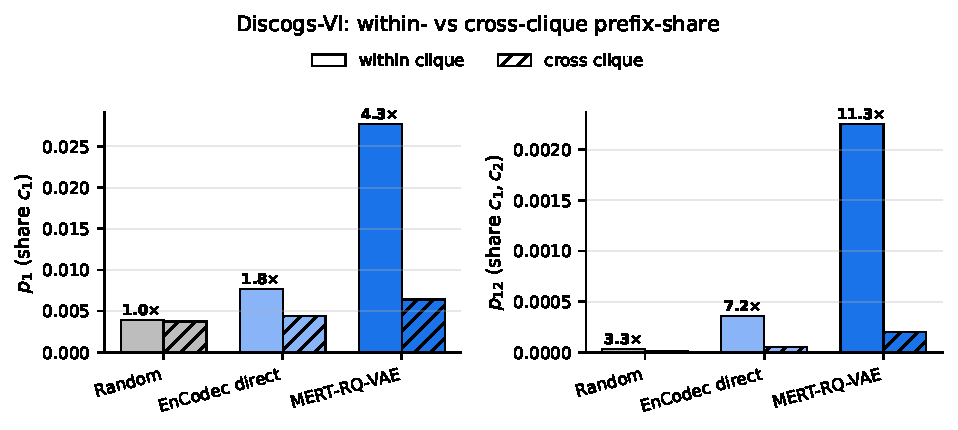
\includegraphics[width=\columnwidth]{figures/prefix_overlap.pdf}
\caption{Within- vs cross-clique prefix-share rates on Discogs-VI for the three SemID conditions. Bar height is the fraction of pairs sharing the indicated prefix; annotated multiplier on each within bar is the within/cross ratio. Random IDs sit at the noise floor (1.06$\times$); MERT-RQ-VAE encodes compositional structure most strongly.}
\label{fig:prefix_overlap}
\end{figure}

Figure~\ref{fig:prefix_overlap} and Table~\ref{tab:semid_quality} summarize the result on Discogs-VI. MERT-RQ-VAE SemIDs share the first prefix \textbf{4.3$\times$} as often within a clique as across, and the first two prefixes \textbf{11$\times$} as often. EnCodec direct codes show a smaller but consistent signal (1.8$\times$ and 7$\times$). Random IDs are within sampling noise of unity. \emph{This structure exists prior to any T5 training}---it is a property of the SemID construction itself.

\begin{table}[t]
\caption{Semantic ID quality on Discogs-VI (3{,}413 tracks). Within/cross is the ratio of prefix-share rates inside vs.\ across cliques. Higher = more compositional structure encoded.}
\label{tab:semid_quality}
\centering
\begin{tabular}{lrrrr}
\toprule
Condition & Clash & Util.\ c1 & W/C $p_1$ & W/C $p_{12}$ \\
\midrule
Random          & 0.0003 & 256/256  & 1.06$\times$ & 3.3$\times$ \\
EnCodec direct  & 0.008  & 578/1024 & 1.8$\times$  & 7.0$\times$ \\
MERT-RQ-VAE     & 0.014  & 256/256  & \textbf{4.3$\times$} & \textbf{11$\times$} \\
\bottomrule
\end{tabular}
\end{table}

\subsection{Cross-Dataset Structure Transfer}
On Covers80, encoded with the same RQ-VAE codebooks trained on Discogs-VI, MERT-RQ-VAE retains $p_1^\text{within} / p_1^\text{cross} = 1.6\times$. The signal is weaker (Covers80 has 80 within-pairs vs.\ 30{,}603 on Discogs-VI, so the variance is high), but the direction is consistent: the SemID structure is not a Discogs-VI artifact.

\begin{figure}[t]
\centering
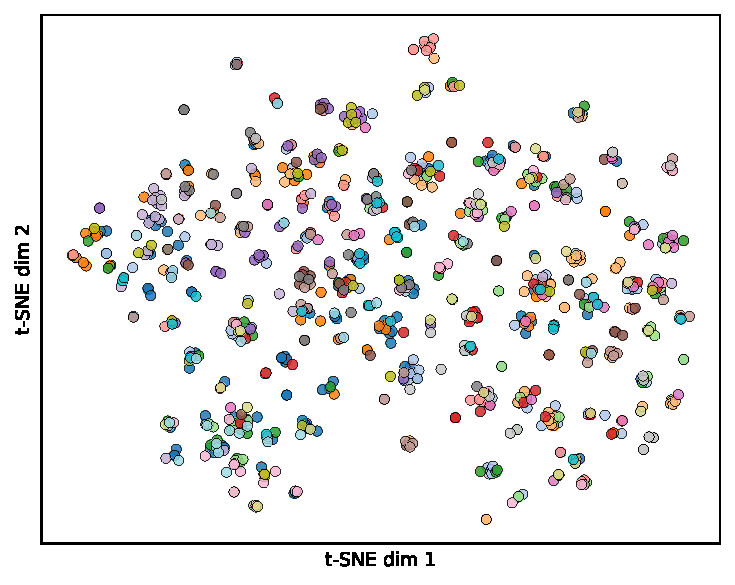
\includegraphics[width=\columnwidth]{figures/tsne.pdf}
\caption{t-SNE projection of MERT-RQ-VAE Semantic IDs (codebook-expanded) for the 20 most-populous Discogs-VI cliques. Tracks within a clique are colored alike; visible coloring suggests that the SemID code space separates cliques to a meaningful extent.}
\label{fig:tsne}
\end{figure}

Figure~\ref{fig:tsne} visualizes the SemID space for the 20 most-populous cliques, projected via t-SNE on the codebook-expanded vectors. Clique coloring is visible as locally coherent regions of the embedding, consistent with the prefix-overlap statistics above.

\subsection{EnCodec Collapses on Low-Bitrate Audio}
The same EnCodec direct codes that show 1.8$\times$ structure on Discogs-VI clean WAVs collapse on Covers80's 32~kbps mp3s: codebook utilization drops to 57/30/29 of 1024 per level, clash rate jumps to 0.41 (95 unique SemIDs for 160 tracks), and within $\approx$ cross prefix-overlap (1.0$\times$ at $p_1$). The low-bitrate spectral content evidently maps to a narrow region of EnCodec's code space, regardless of compositional identity. This is a concrete weakness of using raw codec codes as Semantic IDs and a motivation for the learned-RQ-VAE approach.

\subsection{Main Retrieval Results}
We evaluate generative retrieval in the transductive regime standard to DSI and TIGER: the full corpus is indexed and the train/val/test split is over $(\text{query}\rightarrow\text{cover})$ pairs. Table~\ref{tab:main_results} reports retrieval on the Discogs-VI test set (2{,}324 query tracks).

\begin{table}[t]
\caption{Retrieval on Discogs-VI (2{,}324 query tracks). Bi-encoder is MERT + FAISS; T5 rows are generative retrieval, one model per SemID condition. Best per column in bold.}
\label{tab:main_results}
\centering
\small
\begin{tabular}{lcccccc}
\toprule
Model & MR1 & MRR & MAP & R@1 & R@5 & R@10 \\
\midrule
Bi-encoder (MERT)    & 14.0 & 0.214 & 0.181 & 0.152 & 0.278 & \textbf{0.355} \\
T5 random            & 18.1 & 0.112 & 0.100 & 0.095 & 0.122 & 0.148 \\
T5 EnCodec direct    & 17.9 & 0.122 & 0.106 & 0.102 & 0.140 & 0.150 \\
T5 MERT-RQ-VAE       & \textbf{13.3} & \textbf{0.271} & \textbf{0.254} & \textbf{0.237} & \textbf{0.311} & 0.345 \\
\bottomrule
\end{tabular}
\end{table}

Three findings. First, \textbf{generative retrieval with MERT-RQ-VAE Semantic IDs outperforms the MERT bi-encoder} on five of six metrics, losing only Recall@10 by 0.010. The Recall@1 gain is the largest---0.237 vs.\ 0.152, a 56\% relative improvement---indicating that constrained autoregressive generation yields a sharper top-of-list ranking, while the bi-encoder catches up only in the deep tail.

Second, the condition ordering (random $\approx$ EnCodec $\ll$ MERT-RQ-VAE) is identical to the pre-training prefix-overlap ordering in Table~\ref{tab:semid_quality}. The Semantic ID structure measured before training directly predicts downstream retrieval quality. T5 with random IDs reaches MRR 0.11 by pure memorization of the corpus; structured MERT IDs more than double that.

Third, this replicates the central finding of TIGER~\cite{rajput2023tiger}---structured identifiers far outperform arbitrary ones---and demonstrates it holds for \emph{audio-derived} structure on a real cover song retrieval task.

\subsection{The Transductive Limitation}
Generative retrieval memorizes a fixed corpus: the model's parameters are the index. A model trained on Discogs-VI generates Discogs-VI Semantic IDs and cannot retrieve Covers80 tracks, whose IDs it never indexed---cross-dataset generative retrieval scores zero. This is a property of the paradigm, not a defect of our system, and it is the price paid for eliminating the search index. The bi-encoder, by contrast, handles new catalogs without retraining. We discuss this trade-off further in the limitations.

\section{Limitations and Future Work}
The Discogs-VI subset is constrained by YouTube link rot and bot-detection ($\sim$72\% loss). Recovering bot-detected entries with logged-in cookies is straightforward and would multiply the eval set; we report results on the un-recovered subset to keep the construction reproducible. The model trains and evaluates on 30-second center clips, ignoring longer-form structure that may carry additional compositional cues. The two input modes considered in early planning (SemID-to-SemID and continuous-MERT-to-SemID via a learned projection) reduce to SemID-to-SemID in the current evaluation; we leave the projection variant for future work.

\section{Conclusion}
We have introduced the first generative retrieval system for cover song identification. Audio-derived Semantic IDs from a learned RQ-VAE over MERT embeddings carry strong compositional structure (4.3$\times$/11$\times$ within/cross prefix-overlap), while EnCodec direct codes carry weaker and quality-sensitive structure. A 60M-parameter T5 generating MERT-RQ-VAE Semantic IDs outperforms a MERT bi-encoder on Discogs-VI retrieval (MRR 0.271 vs.\ 0.214), with the three SemID conditions ranking exactly as their pre-training structure predicts. The approach is transductive---it cannot retrieve un-indexed catalogs---which is the principled cost of replacing the search index with model parameters. Future work includes recovering the bot-blocked portion of the crawl for a larger corpus, the continuous-MERT-to-SemID input variant, and an indexing objective that could relax the transductive constraint.

\begin{thebibliography}{00}
\bibitem{tay2022dsi} Y. Tay et al., ``Transformer memory as a differentiable search index,'' in \emph{NeurIPS}, 2022.
\bibitem{rajput2023tiger} S. Rajput et al., ``Recommender systems with generative retrieval,'' in \emph{NeurIPS}, 2023.
\bibitem{palumbo2025text2tracks} E. Palumbo and G. Penha, ``Text2Tracks: prompt-based music recommendation via generative retrieval,'' \emph{arXiv:2503.24193}, 2025.
\bibitem{kim2026fusid} M. Kim, T. Hou, and J. McAuley, ``FusID: multimodal fused semantic IDs for music recommendation,'' \emph{arXiv:2601.08764}, 2026.
\bibitem{mei2025semids} M. Mei et al., ``Semantic IDs for music recommendation at scale,'' in \emph{RecSys}, 2025.
\bibitem{yuan2023mert} Y. Yuan et al., ``MERT: acoustic music understanding model with large-scale self-supervised training,'' \emph{arXiv:2306.00107}, 2023.
\bibitem{defossez2022encodec} A. D{\'e}fossez et al., ``High fidelity neural audio compression,'' \emph{arXiv:2210.13438}, 2022.
\bibitem{araz2024discogsvi} R. O. Araz, X. Serra, and D. Bogdanov, ``Discogs-VI: a musical version identification dataset based on public editorial metadata,'' in \emph{ISMIR}, 2024.
\bibitem{yesiler2019datacos} F. Yesiler et al., ``Da-TACOS: a dataset for cover song identification and understanding,'' in \emph{ISMIR}, 2019.
\bibitem{ellis2007covers80} D. P. W. Ellis, ``The ``covers80'' cover song dataset,'' Tech.\ Rep., Columbia University LabROSA, 2007.
\bibitem{yesiler2019move} F. Yesiler, J. Serr{\`a}, and E. G{\'o}mez, ``Accurate and scalable version identification using musically-motivated embeddings,'' in \emph{ICASSP}, 2020.
\bibitem{doh2021coverhunter} S. Doh et al., ``CoverHunter: cover song identification with refined attention and alignments,'' in \emph{ISMIR}, 2021.
\bibitem{lee2022rqvae} D. Lee et al., ``Autoregressive image generation using residual quantization,'' in \emph{CVPR}, 2022.
\bibitem{zeghidour2021soundstream} N. Zeghidour et al., ``SoundStream: an end-to-end neural audio codec,'' \emph{arXiv:2107.03312}, 2021.
\bibitem{raffel2020t5} C. Raffel et al., ``Exploring the limits of transfer learning with a unified text-to-text transformer,'' \emph{JMLR}, vol.~21, 2020.
\end{thebibliography}

\end{document}
